\documentclass[11pt]{beamer}
\usetheme{Bergen}
\usecolortheme{albatross}
\usefonttheme{serif}
\usepackage[english]{babel}
\usepackage{amsmath}
\usepackage{amsfonts}
\usepackage{amssymb}
\usepackage{graphicx}
\usepackage{listings}
\usepackage{fontspec}
\setmainfont[Ligatures=TeX]{Noto Sans}
\setmonofont[Ligatures=TeX]{Noto Sans Mono}

\author{Raphael Emberger}
\title{San Francisco Crime Classification}
%\setbeamercovered{transparent}
%\setbeamertemplate{navigation symbols}{}
%\logo{}
\institute{NUT}
\date{\today}
\subject{Crime classification}

% https://terminal.sexy/
% Export as MinTTY
% Regex-replace:
% ^([^=]+)=(.+)$
% \definecolor{$1}{RGB}{$2}
% Or:
\usepackage{xcolor}
%\usepackage{termcol}
%\loadcolors{terminalcolors2}
\definecolor{BackgroundColour}{RGB}{29,31,33}
\definecolor{ForegroundColour}{RGB}{197,200,198}
\definecolor{CursorColour}{RGB}{197,200,198}
\definecolor{Black}{RGB}{40,42,46}
\definecolor{BoldBlack}{RGB}{55,59,65}
\definecolor{Red}{RGB}{165,66,66}
\definecolor{BoldRed}{RGB}{204,102,102}
\definecolor{Green}{RGB}{140,148,64}
\definecolor{BoldGreen}{RGB}{181,189,104}
\definecolor{Yellow}{RGB}{222,147,95}
\definecolor{BoldYellow}{RGB}{240,198,116}
\definecolor{Blue}{RGB}{95,129,157}
\definecolor{BoldBlue}{RGB}{129,162,190}
\definecolor{Magenta}{RGB}{133,103,143}
\definecolor{BoldMagenta}{RGB}{178,148,187}
\definecolor{Cyan}{RGB}{94,141,135}
\definecolor{BoldCyan}{RGB}{138,190,183}
\definecolor{White}{RGB}{112,120,128}
\definecolor{BoldWhite}{RGB}{197,200,198}

%collection/hybrid
%base16/atelierforest.light
%xcolors.net/euphrasia
%collection/hund
%collection/dawn

\setbeamercolor*{normal text}{
	fg=ForegroundColour,
	bg=BackgroundColour
}\setbeamercolor*{structure}{
	fg=Red
}
\setbeamersize{sidebar width left=.15\paperwidth}

\lstset{
	frame=none,
%	aboveskip=3mm,
%	belowskip=3mm,
	captionpos=b,
	showstringspaces=false,
	breaklines=true,
	breakatwhitespace=true,
	postbreak=\mbox{\textcolor{Red}{$\hookrightarrow$}\space},
%	tabsize=4,
	keepspaces=false,
	columns=flexible,
	escapeinside={\%*}{*)},
	otherkeywords={},
	deletekeywords={},
	numbers=left,
	numbersep=10pt,
	numberstyle=\color{BackgroundColour!95!ForegroundColour},
	%% Colors and fonts:
	basicstyle=\footnotesize\ttfamily\color{ForegroundColour!70!BackgroundColour},
	numberstyle=\tiny\color{ForegroundColour},
	keywordstyle=\color{Blue},
	commentstyle=\color{BoldGreen},
    identifierstyle=\color{ForegroundColour},
	stringstyle=\color{Red},
	backgroundcolor=\color{BackgroundColour!90!ForegroundColour},
	rulecolor=\color{Black}
}

\begin{document}

\begin{frame}
\centering
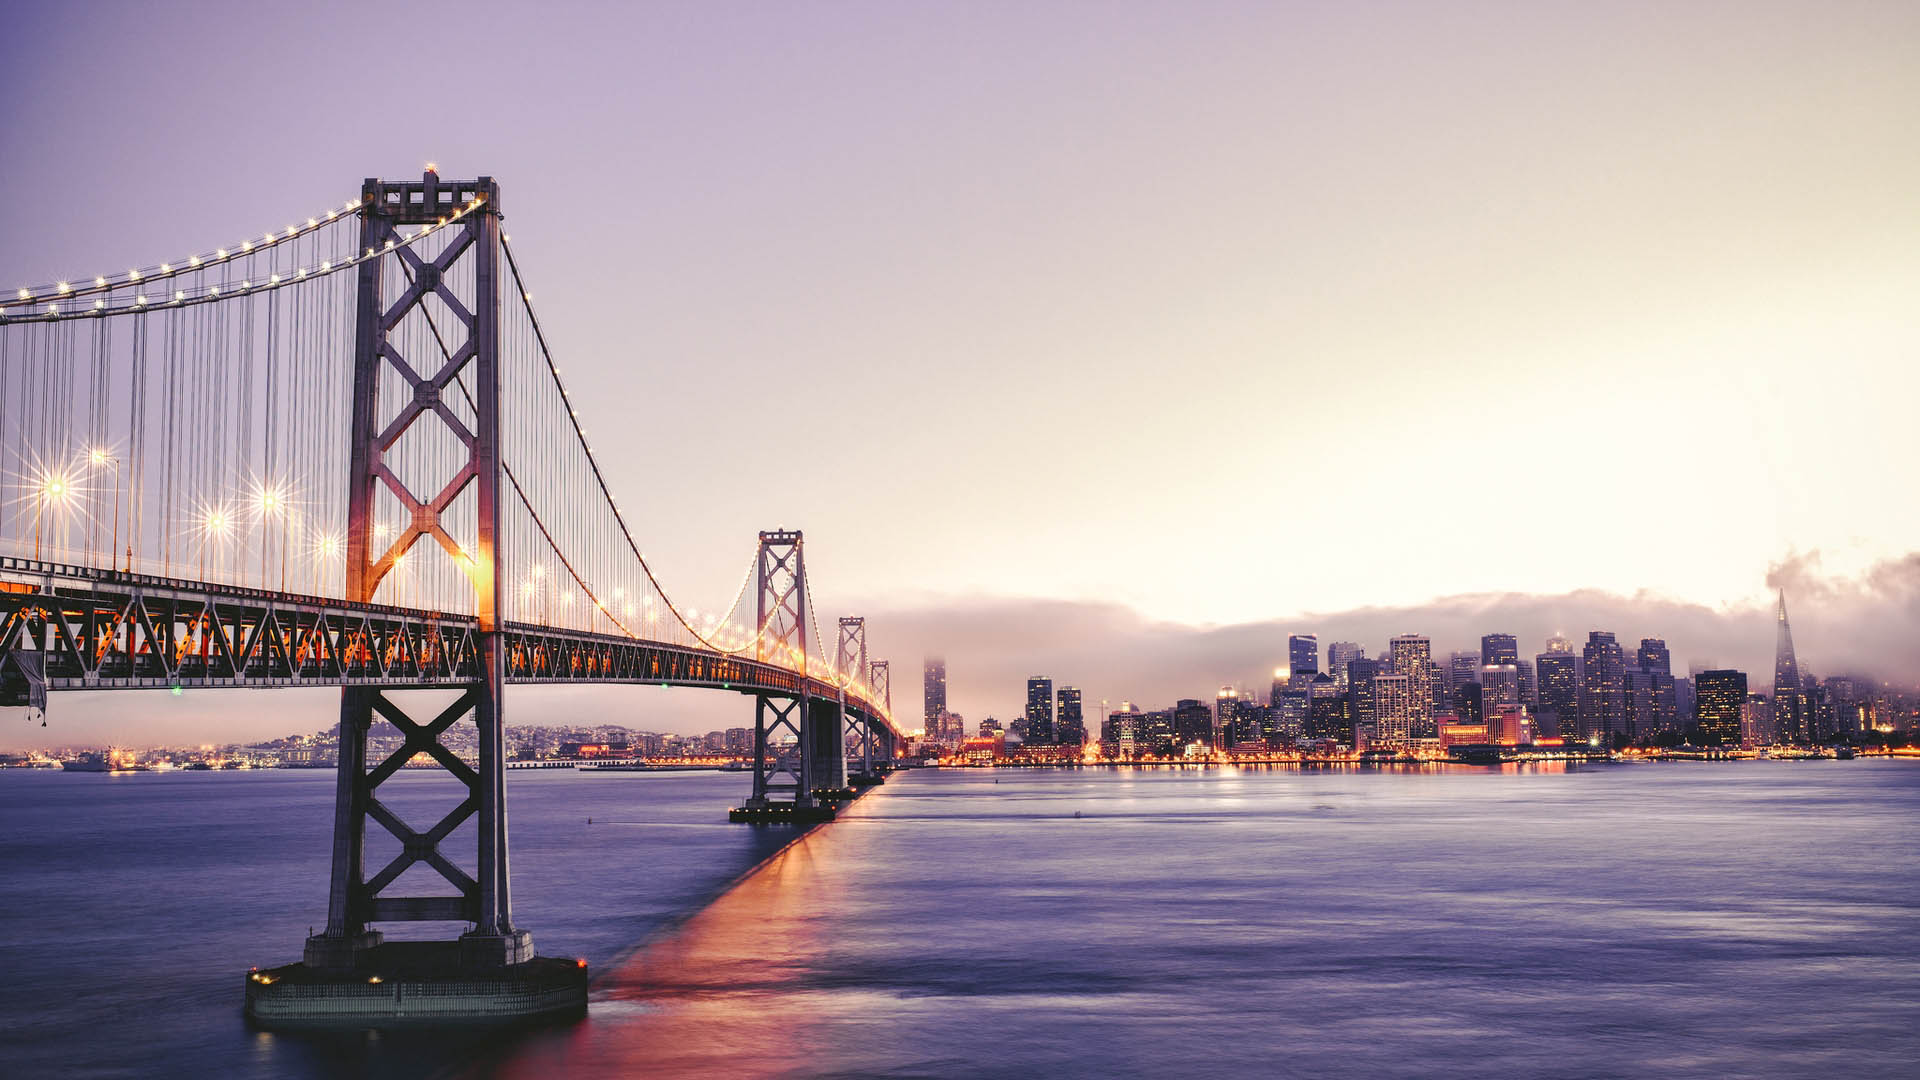
\includegraphics[width=\textwidth]{San-Francisco}
\titlepage
\end{frame}

\begin{frame}{Challenge}
Classify type of crime using:
\begin{itemize}
\item Date-time
\item Weekday
\item District name
\item Address
\item Latitude
\item Longitude
\end{itemize}
into 39 labels.

Dataset from 2003 - 2015
\end{frame}

\begin{frame}{Map of Crimes}
\centering
\includegraphics[width=\textwidth]{sf_top_crimes_map}
\end{frame}

\begin{frame}{Ranking}
\begin{itemize}
\item Soft-max
\item Log-loss:
\begin{align}\label{eqn:loss}
&loss = -\frac1N\sum_{i=1}^N{\color{Red}\sum_{j=1}^My_{ij}\log\left(p_{ij}\right)}\\
\nonumber
N: & \hspace{8pt} \textrm{Number of cases in dataset.}\\
\nonumber
M: & \hspace{8pt} \textrm{Number of classes.}\\
\nonumber
y_{ij}: & \hspace{8pt} \textrm{Label for class. 1 if $i$ is in $j$. Otherwise 0.}\\
\nonumber
p_{ij}: & \hspace{8pt} \textrm{Predicted probability that $i$ belongs to $j$.}
\end{align}
\item 2335 submissions
\item 34.53877 - 1.95936
\item Rank 2241: 32.89183
\end{itemize}
\end{frame}

\begin{frame}{Dataset}
\begin{itemize}
\item \textbf{sampleSubmission.csv}(884k x 40)
\item \textbf{test.csv}(884k x 7)
\item \textbf{train.csv}(878k x 9)
\end{itemize}
\end{frame}

\begin{frame}{Train Dataset}
\begin{table}[htbp]
\centering
\tiny
\setlength\tabcolsep{2pt}
\begin{tabular}{|ccccc}\hline
Dates&Category&Descript&DayOfWeek&PdDistrict\\\hline\hline
2015-05-13 23:53:00&WARRANTS&WARRANT ARREST&Wednesday&NORTHERN\\
2015-05-13 23:53:00&OTHER OFFENSES&TRAFFIC VIOLATION ARREST&Wednesday&NORTHERN\\
2015-05-13 23:33:00&OTHER OFFENSES&TRAFFIC VIOLATION ARREST&Wednesday&NORTHERN\\
2015-05-13 23:30:00&LARCENY/THEFT&GRAND THEFT FROM LOCKED AUTO&Wednesday&NORTHERN\\
2015-05-13 23:30:00&LARCENY/THEFT&GRAND THEFT FROM LOCKED AUTO&Wednesday&PARK\\
2015-05-13 23:30:00&LARCENY/THEFT&GRAND THEFT FROM UNLOCKED AUTO&Wednesday&INGLESIDE\\
2015-05-13 23:30:00&VEHICLE THEFT&STOLEN AUTOMOBILE&Wednesday&INGLESIDE\\
2015-05-13 23:30:00&VEHICLE THEFT&STOLEN AUTOMOBILE&Wednesday&BAYVIEW\\
2015-05-13 23:00:00&LARCENY/THEFT&GRAND THEFT FROM LOCKED AUTO&Wednesday&RICHMOND\\
2015-05-13 23:00:00&LARCENY/THEFT&GRAND THEFT FROM LOCKED AUTO&Wednesday&CENTRAL\\\hline
\end{tabular}

\begin{tabular}{cccc|}\hline
Resolution&Address&X&Y\\\hline\hline
"ARREST, BOOKED"&OAK ST / LAGUNA ST&-122.425891675136&37.7745985956747\\
"ARREST, BOOKED"&OAK ST / LAGUNA ST&-122.425891675136&37.7745985956747\\
"ARREST, BOOKED"&VANNESS AV / GREENWICH ST&-122.42436302145&37.8004143219856\\
NONE&1500 Block of LOMBARD ST&-122.42699532676599&37.80087263276921\\
NONE&100 Block of BRODERICK ST&-122.438737622757&37.771541172057795\\
NONE&0 Block of TEDDY AV&-122.40325236121201&37.713430704116\\
NONE&AVALON AV / PERU AV&-122.423326976668&37.7251380403778\\
NONE&KIRKWOOD AV / DONAHUE ST&-122.371274317441&37.7275640719518\\
NONE&600 Block of 47TH AV&-122.508194031117&37.776601260681204\\
NONE&JEFFERSON ST / LEAVENWORTH ST&-122.419087676747&37.8078015516515\\\hline
\end{tabular}
\caption{train.csv(first 10 rows)}
\label{tab:train.csv}
\end{table}
\end{frame}

\begin{frame}{Test Dataset}
\begin{table}[htbp]
\centering
\scriptsize
\setlength\tabcolsep{2pt}
\begin{tabular}{|ccccc}\hline
Id&Dates&DayOfWeek&PdDistrict&Address\\\hline\hline
0&2015-05-10 23:59:00&Sunday&BAYVIEW&2000 Block of THOMAS AV\\
1&2015-05-10 23:51:00&Sunday&BAYVIEW&3RD ST / REVERE AV\\
2&2015-05-10 23:50:00&Sunday&NORTHERN&2000 Block of GOUGH ST\\
3&2015-05-10 23:45:00&Sunday&INGLESIDE&4700 Block of MISSION ST\\
4&2015-05-10 23:45:00&Sunday&INGLESIDE&4700 Block of MISSION ST\\
5&2015-05-10 23:40:00&Sunday&TARAVAL&BROAD ST / CAPITOL AV\\
6&2015-05-10 23:30:00&Sunday&INGLESIDE&100 Block of CHENERY ST\\
7&2015-05-10 23:30:00&Sunday&INGLESIDE&200 Block of BANKS ST\\
8&2015-05-10 23:10:00&Sunday&MISSION&2900 Block of 16TH ST\\
9&2015-05-10 23:10:00&Sunday&CENTRAL&TAYLOR ST / GREEN ST\\\hline
\end{tabular}
\begin{tabular}{cc|}\hline
X&Y\\\hline\hline
-122.39958770418998&37.7350510103906\\
-122.391522893042&37.7324323864471\\
-122.426001954961&37.7922124386284\\
-122.437393972517&37.7214120621391\\
-122.437393972517&37.7214120621391\\
-122.45902362242902&37.7131719025215\\
-122.42561645123001&37.73935051446279\\
-122.41265203979201&37.739750156312105\\
-122.418700097043&37.7651649409646\\
-122.413934584561&37.798886450641604\\\hline
\end{tabular}
\caption{test.csv(first 10 rows)}
\label{tab:test.csv}
\end{table}
\end{frame}

\begin{frame}{Labels}
\begin{table}[htbp]
\centering
\tiny
\setlength\tabcolsep{2pt}
\begin{tabular}{|lll|}\hline
ARSON&ASSAULT&BAD CHECKS\\
BRIBERY&BURGLARY&DISORDERLY CONDUCT\\
DRIVING UNDER THE INFLUENCE&DRUG/NARCOTIC&DRUNKENNESS\\
EMBEZZLEMENT&EXTORTION&FAMILY OFFENSES\\
FORGERY/COUNTERFEITING&FRAUD&GAMBLING\\
KIDNAPPING&LARCENY/THEFT&LIQUOR LAWS\\
LOITERING&MISSING PERSON&NON-CRIMINAL\\
OTHER OFFENSES&PORNOGRAPHY/OBSCENE MAT&PROSTITUTION\\
RECOVERED VEHICLE&ROBBERY&RUNAWAY\\
SECONDARY CODES&SEX OFFENSES FORCIBLE&SEX OFFENSES NON FORCIBLE\\
STOLEN PROPERTY&SUICIDE&SUSPICIOUS OCC\\
TREA&TRESPASS&VANDALISM\\
VEHICLE THEFT&WARRANTS&WEAPON LAWS\\
\hline
\end{tabular}
\caption{Crime classes}
\label{tab:lables}
\end{table}
\end{frame}

\begin{frame}{First Approach}
\begin{itemize}
\item Keras model
\item Preprocessing:
\begin{itemize}
\item Conversion to integer/float
\item Feature scaling
\item Mean normalization
\end{itemize}
\item OOP
\item Caching
\end{itemize}
\end{frame}

\begin{frame}{First Approach}
\lstinputlisting[language=python, firstline=28, firstnumber=28, lastline=41,label=lst:keras_model,caption={Keras model - model.py}]{../model.py}
\end{frame}

\begin{frame}{First Approach(last one, I swear)}
\lstinputlisting[language=python, firstline=34, firstnumber=34, lastline=55, label=lst:main_py, caption={Classification process(first approach) - main.py}, basicstyle=\tiny\ttfamily\color{ForegroundColour!70!BackgroundColour}]{../main.py}
\end{frame}

\begin{frame}[fragile]{Results}
\begin{itemize}
\item Rank 1058
\item Accuracy converges to ca. 19.9\%
\item Mostly assumes "Larceny/Theft"(19.92\% of the Dataset)
\item Tempering with parameters has no effect
\item Different approach required
\end{itemize}
\end{frame}

\begin{frame}{Second Approach}
\begin{itemize}
\item Ramunno-Johnson's blog
\item Bernoulli Naïves Bayes(Linear Regression for comparison)
\item Preprocessing: Binarization
\begin{itemize}
\item Minutes(m0 - m59)
\item Hours(H1 - H12)
\item Days(D1 - D31)
\item Months(M1 - M12)
\item Years(Y2003 - Y2015)
\item Weekdays(Monday - Sunday)
\item Districts(Bayview - Tenderloin)
\end{itemize}
\end{itemize}
\end{frame}

\begin{frame}{Second Approach}
\lstinputlisting[language=python, firstline=30, firstnumber=30, lastline=50,label=lst:newmain_py_preprocess,caption={Pre-processing method - newmain.py}, basicstyle=\tiny\ttfamily\color{ForegroundColour!70!BackgroundColour}]{../newmain.py}
$\Rightarrow$ simpler script
\end{frame}

\begin{frame}{Second Approach(Bernoulli Naïves Bayes)}
\lstinputlisting[language=python, firstline=53, firstnumber=53, lastline=82,label=lst:newmain_py_bnb,caption={Bernoulli Naïve Bayes fitting- newmain.py}, basicstyle=\tiny\ttfamily\color{ForegroundColour!70!BackgroundColour}]{../newmain.py}
\end{frame}

\begin{frame}{Results}
\begin{itemize}
\item Rank 675(before: 1058)
\item Log-loss: 2.464(26.02\%)
\item Logistic Regression on rank 1149
\item Log-loss: 2.591(24.43\%)
\end{itemize}
\end{frame}

\begin{frame}{Third Approach}
\begin{itemize}
\item Keras model
\item Combine
\item Preprocessing: Same binarization
\end{itemize}
\end{frame}

\begin{frame}[fragile]{Third Approach}
\lstinputlisting[language=python, firstline=100, firstnumber=100, lastline=116,label=lst:newmain_py_keras,caption={Keras model integrated - newmain.py}]{../newmain.py}
\end{frame}

\begin{frame}{Results}
\begin{itemize}
\item Rank 664(before: 675)
\item Log-loss: 2.456(26.39\%) - before: 2.464(26.02\%)
\end{itemize}
\end{frame}

\begin{frame}{Conclusion and Future Considerations}
Mistakes made:
\begin{itemize}
\item Too much time invested into first approach
\item Too little knowledge and experience with NNs
\end{itemize}
\vspace{1cm}
Potential next steps:
\begin{itemize}
\item Gathering knowledge about NNs
\item Enrich dataset
\item Even out the dataset
\end{itemize}
\end{frame}

\begin{frame}{End of Presentation}
\vfill
\centering
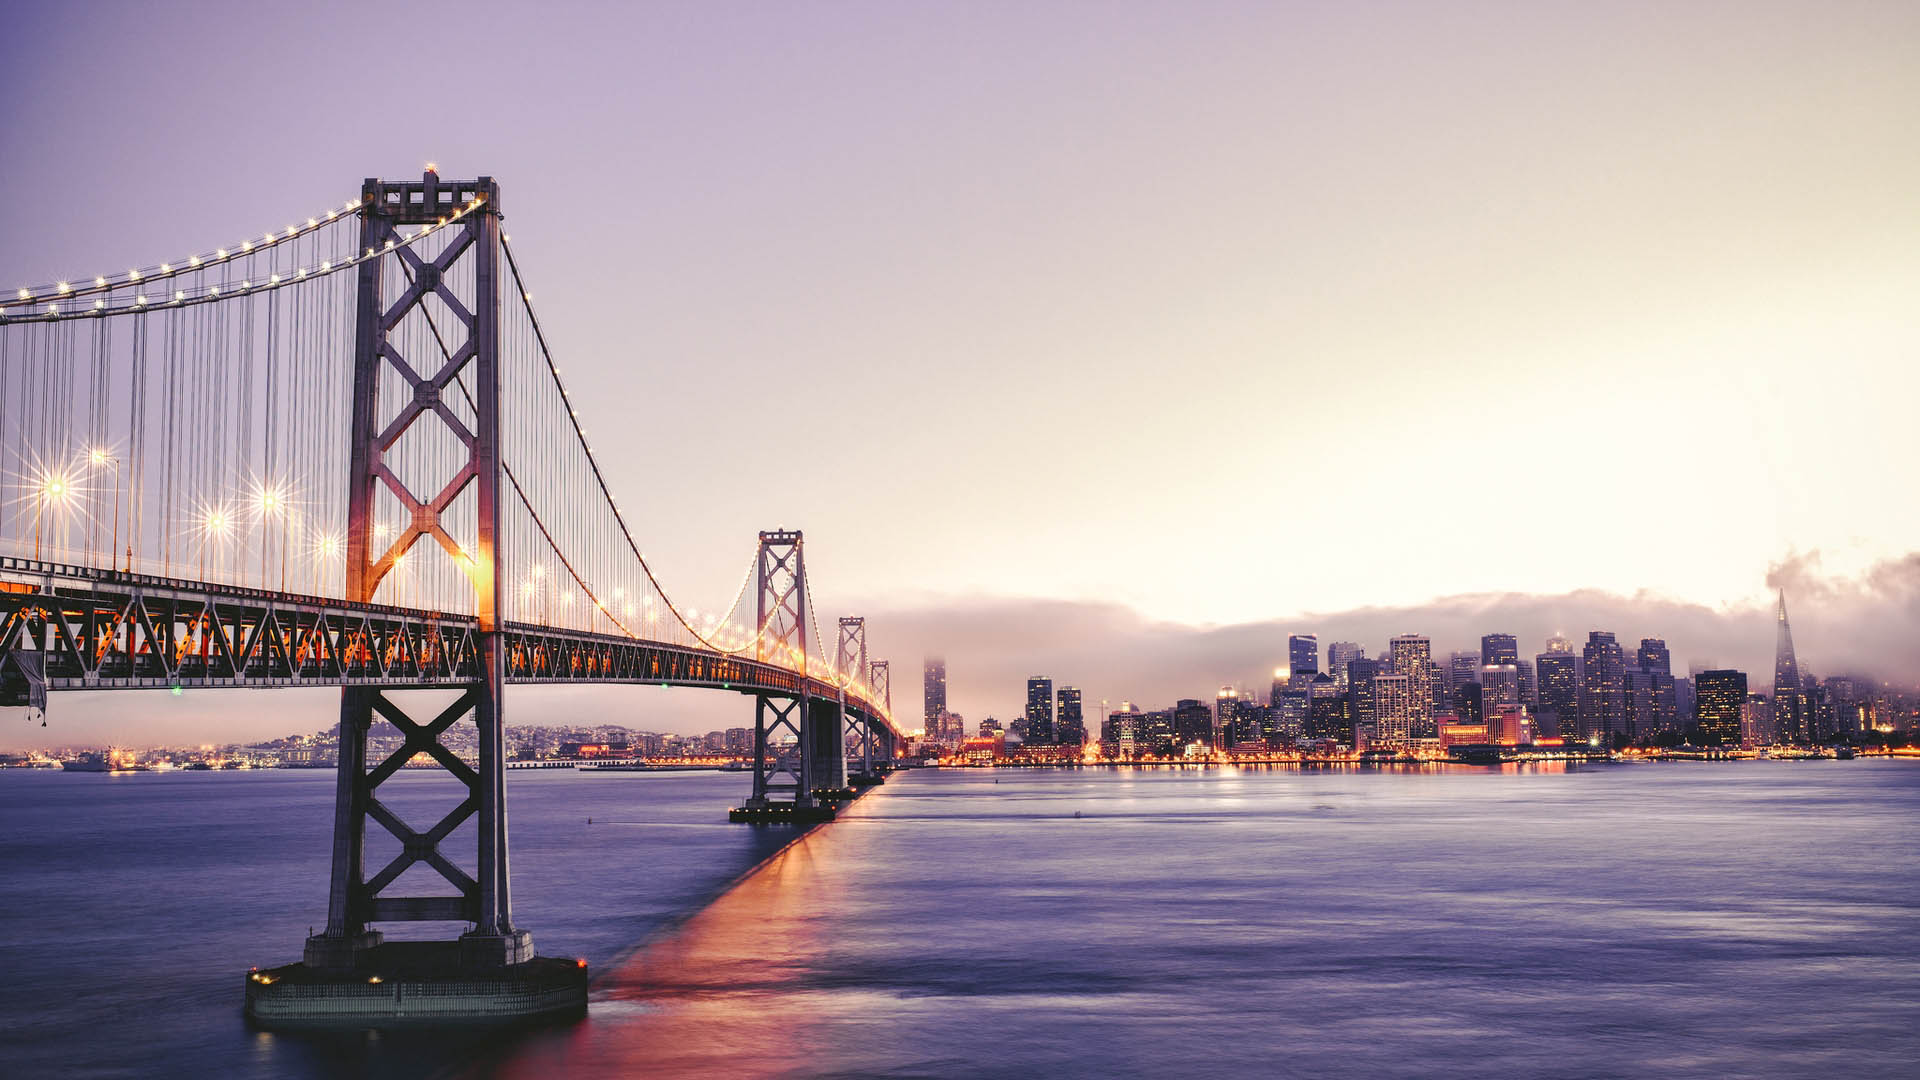
\includegraphics[width=\textwidth]{San-Francisco}
Thank you for your attention
\vfill
\end{frame}

\end{document}